%//////////////////////////////////
%/// P R E A M B L E

\documentclass[a4paper, 12pt]{article}

\usepackage[utf8]{inputenc}
\usepackage[singlespacing]{setspace}
\usepackage{amsmath}
\usepackage{mathtools}
\usepackage{caption}
\usepackage{float}
\usepackage{graphicx}
\usepackage{multicol}
\usepackage{gensymb}
\usepackage{breqn}
\usepackage{indentfirst}
\usepackage{siunitx}
\usepackage{tabularx, booktabs}
\newcolumntype{Y}{>{\centering\arraybackslash}X}

\usepackage{pdfpages}

\usepackage{multicol}
\usepackage{supertabular}

\usepackage{svg}

\widowpenalty = 4500
\clubpenalty  = 4500

\setlength{\jot}{10pt} %indents


\newcommand*\dif{\mathop{}\!\mathrm{d}}
%\newcommand{\euler}{\mathrm{e}}
%\newcommand{\ramuno}{\mathrm{j}}

%%========================================
%% circuitikz properties
\usepackage[european, straightvoltages]{circuitikz}
%\ctikzvalof{voltage/distance from node = .2}
%\ctikzset{voltage/distance from node  =.5}% in \pgf@circ@Rlen units
%\ctikzset{voltage/distance from line  =.25}% pos. between 0 and 1
%\ctikzset{voltage/bump b/.initial     =1.5}%

\ctikzset{current/distance            = .618}


%%========================================

%%
%% Path settings
%%
\graphicspath{ {./graphics/} }


%//////////////////////////////////
%/// D O C U M E N T
\begin{document}

%%%%%%%%%%%%%%%%%%%%%%%%%%%%%%%%%%%%%
  %\includepdf{Deckblatt.pdf}
  
\includepdf{./titlepage/titlepage.pdf}
%%%%%%%%%%%%%%%%%%%%%%%%%%%%%%%%%%%%%

\section{Vorbereitungsaufgaben}

  %1.1
  \subsection{}
    \begin{center}
      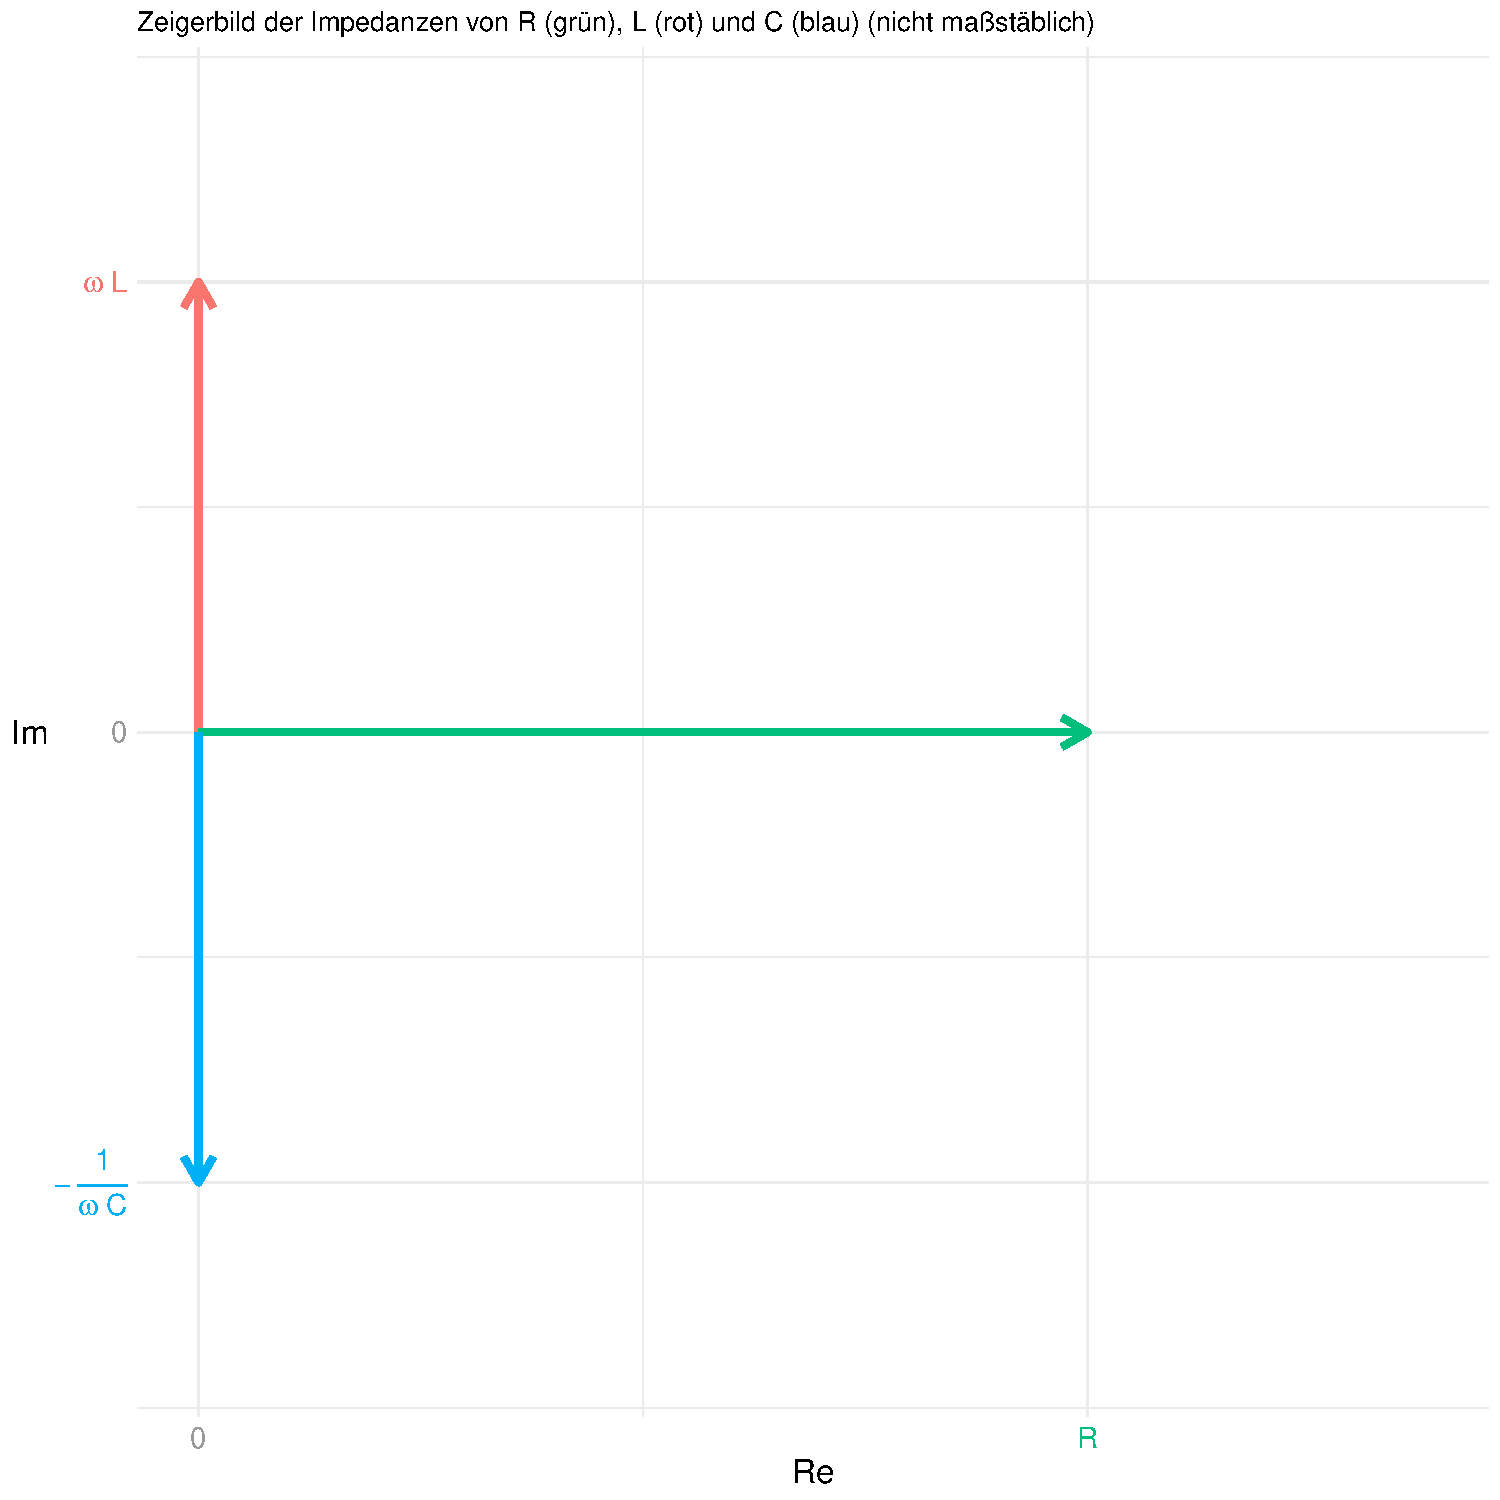
\includegraphics[scale=0.5]{./R/2_1/RLC_Zeiger_Impedanz.pdf}\\
      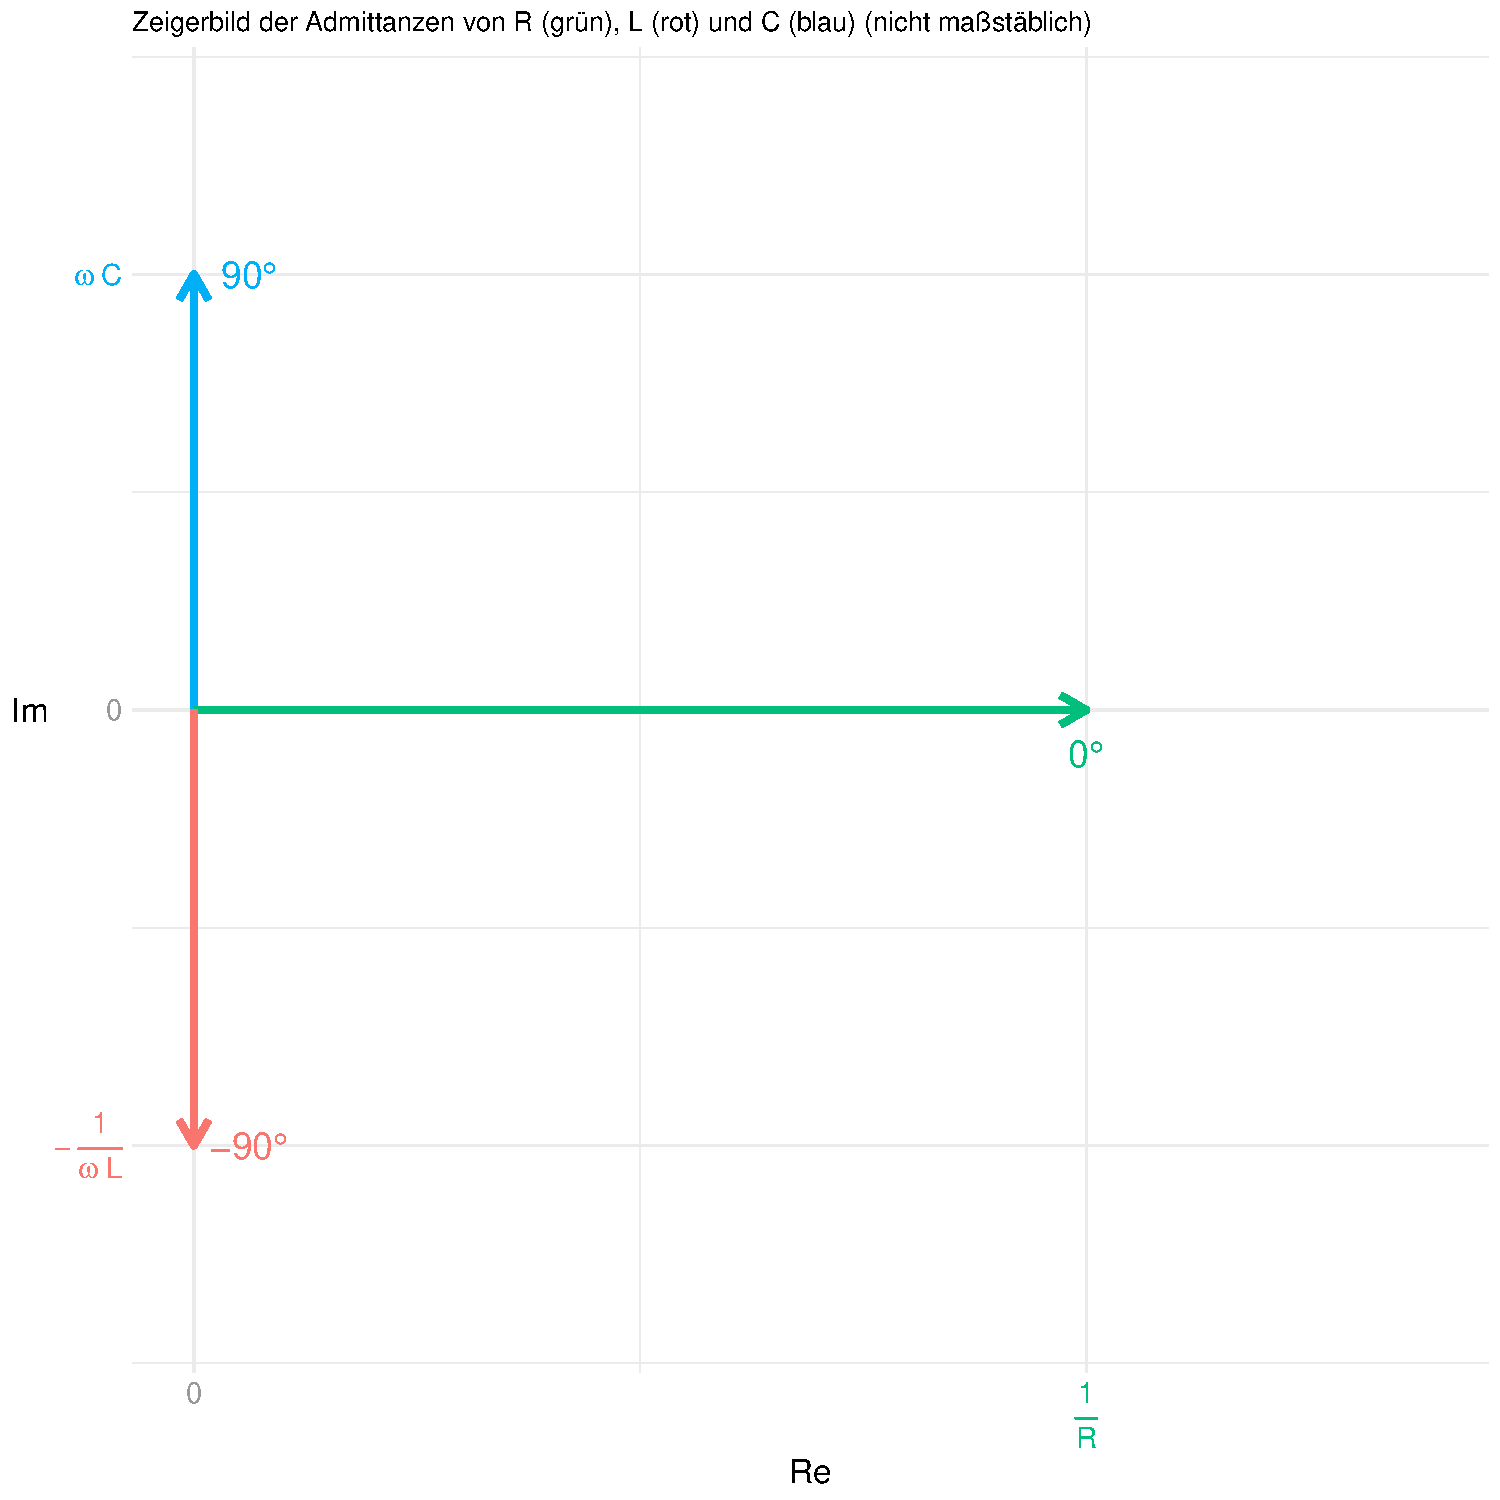
\includegraphics[scale=0.5]{./R/2_1/RLC_Zeiger_Admittanz.pdf}
    \end{center}

  %1.2
  \subsection{}

    \begin{center}
      \begin{circuitikz}

        \draw (0,0) to[R, l=$R$, o-] (2,0);
        \draw (2,0) to[L, l=$L$, i=$\underline{I}$] (6,0);
        \draw (6,0) to[C, l=$C$, -o] (8,0);

      \end{circuitikz}
    \end{center}

    \begin{gather*}
      \underline{I} = \frac{\underline{U}}{\underline{Z}},\,\ \underline{U} = \hat{U} \cdot e^{j(\omega t + \phi_u)}\\
      \underline{Z} = R + j \omega L + \frac{1}{j \omega C}\\
      \underline{I} = \frac{\hat{U} \cdot e^{j(\omega t + \phi_u)}}{R+j (\omega L - \frac{1}{ \omega C})}
      \intertext{Betrag:}
      \mid \underline{I} \mid = \hat{I} = \frac{\hat{U}}{\sqrt{R^2 + (\omega L - \frac{1}{\omega C} )^2}}
      \intertext{Phase:}
      \phi_i = \phi_u - \arctan{\left(\frac{\omega L - \frac{1}{\omega C} }{R} \right)}
      \intertext{Gesamt:}
      i(t) = \frac{\hat{U}}{\sqrt{R^2 + (\omega L - \frac{1}{\omega C} )^2}} \cdot \cos{\left( \omega t +  \phi_u - \arctan{\left(\frac{\omega L - \frac{1}{\omega C} }{R} \right)}\right)}
    \end{gather*}

  %1.3
  \subsection{}
    \begin{center}
      \begin{circuitikz}

        \draw (0,0) to[R, l=$R_{sL}$,v=$U_{R_{\text{eff}}}$, o-] (2,0)
        to[L, l=$L$, -o, v=$U_{L_{\text{eff}}}$, i=$i_{\text{eff}}$] (4,0);

      \end{circuitikz}
      \vspace{0.021276873\paperheight}
    $$I = 1.5 \,\ \si{\milli\ampere}, \,\ R_{sL}=200 \si{\ohm},\,\ L = 60 \,\ \si{\milli\henry}$$ \end{center}

    \begin{gather*}
      \underline{U}_{\text{ges}}=\underline{I}\cdot(R_{sL}+j \omega L)\\
      \hat{U}_{\text{ges}} = \hat{I} \cdot \sqrt{R_{sL}^2 + \omega^2 L^2}\\
      \hat{U}_{\text{ges}_{\text{eff}}}
      = I_{\text{eff}}\cdot \sqrt{R_{sL}^2 + \omega^2 L^2}
      = 1.5 \si{\milli\ampere} \cdot \sqrt{(200 \si{\ohm})^2 + 4 \pi^2 f^2 \cdot (60 \si{\milli\henry})^2 }
    \end{gather*}

    \begin{gather*}
      U_{R_{\text{eff}}} = I_{\text{eff}} \cdot R = 1.5 \si{\milli\ampere} \cdot 200 \si{\ohm} = 0.3 \,\ \si{\volt}
    \end{gather*}

    \begin{gather*}
      U_{L_{\text{eff}}} = I_{\text{eff}} \cdot \omega L = 1.5 \si{\milli\ampere} \cdot 2 \pi f \cdot 60 \si{\milli\henry}
    \end{gather*}

    \begin{center}
      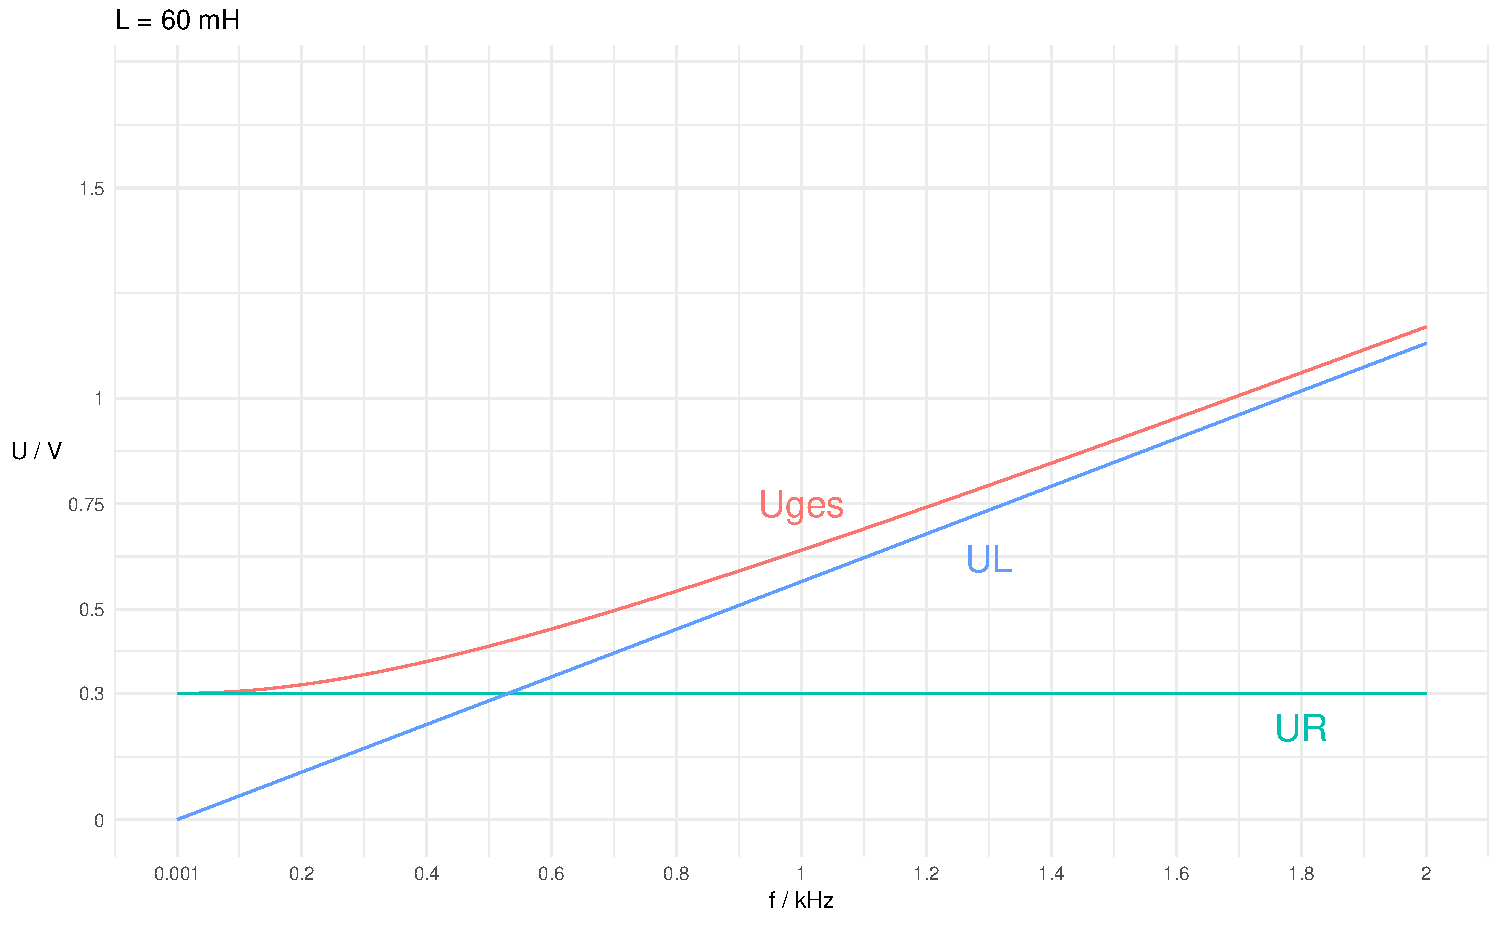
\includegraphics[scale=0.5]{./R/2_3/2_3.pdf}
    \end{center}

  %1.4
  \subsection{}
    \begin{center}
      \begin{circuitikz}

        \draw (0,0) to[R, l=$R$,v=$U_{R_{\text{eff}}}$, o-] (2,0)
        to[C, l=$C$, -o, v=$U_{C_{\text{eff}}}$, i=$i_{\text{eff}}$] (4,0);

      \end{circuitikz}
      \vspace{0.021276873\paperheight}
      $$I = 1.5 \,\ \si{\milli\ampere}, \,\ R=200 \si{\ohm},\,\ C_1 = 0.5 \,\ \si{\micro\farad}, \,\ C_2 = 1 \,\ \si{\micro\farad}$$\end{center}

    \begin{gather*}
      \underline{U}_{\text{ges}}=\underline{I}\cdot(R-j\frac{1}{\omega C})\\
      \hat{U}_{\text{ges}} = \hat{I} \cdot \sqrt{R^2 + \frac{1}{\omega^2 C^2} }\\
      \hat{U}_{\text{ges}_{\text{eff}}}=I_{\text{eff}}\cdot\sqrt{R^2 + \frac{1}{\omega^2 C^2} } = 1.5 \si{\milli\ampere} \cdot \sqrt{(200 \si{\ohm})^2 + \frac{1}{4 \pi^2 f^2 C^2} }
    \end{gather*}

    \begin{gather*}
      U_{R_{\text{eff}}} = I_{\text{eff}} \cdot R = 1.5 \si{\milli\ampere} \cdot 200 \si{\ohm} = 0.3 \,\ \si{\volt}
    \end{gather*}

    \begin{gather*}
        U_{C_{\text{eff}}} = I_{\text{eff}} \cdot \frac{1}{\omega C}\\
        U_{C_{{\text{eff}}_1}} = I_{\text{eff}} \cdot \frac{1}{\omega C_1} = 1.5 \si{\milli\ampere} \cdot \frac{1}{2 \pi f \cdot 0.5 \si{\micro\farad}}\\
        U_{C_{{\text{eff}}_2}} = I_{\text{eff}} \cdot \frac{1}{\omega C_2} = 1.5 \si{\milli\ampere} \cdot \frac{1}{2 \pi f \cdot 1 \si{\micro\farad}}
    \end{gather*}

    \begin{center}
      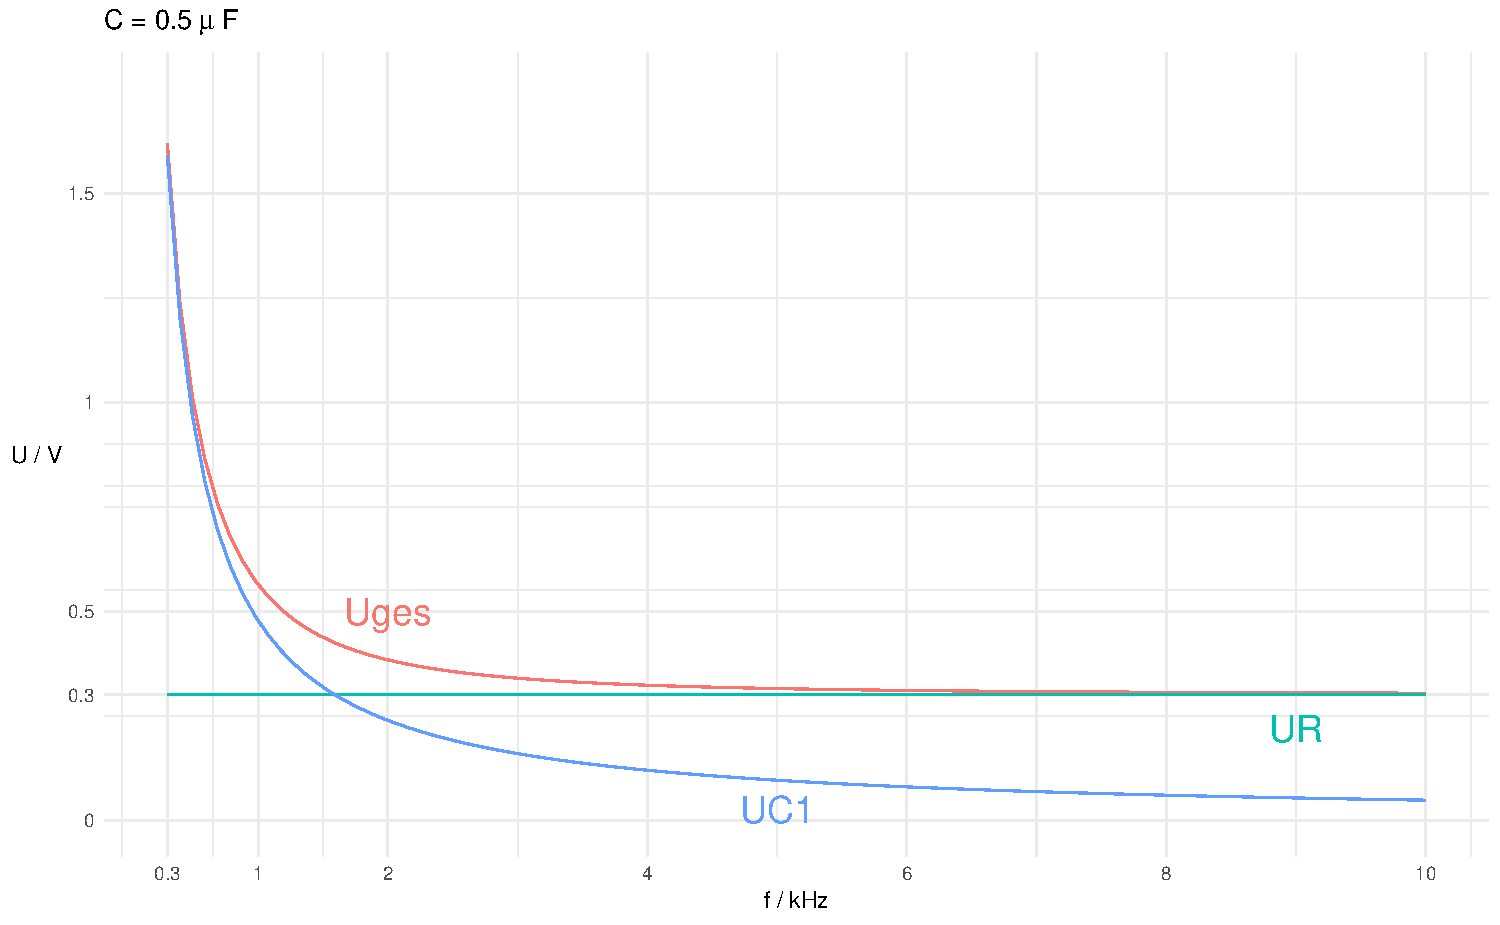
\includegraphics[scale=0.5]{./R/2_4/2_4_1.pdf}\\
      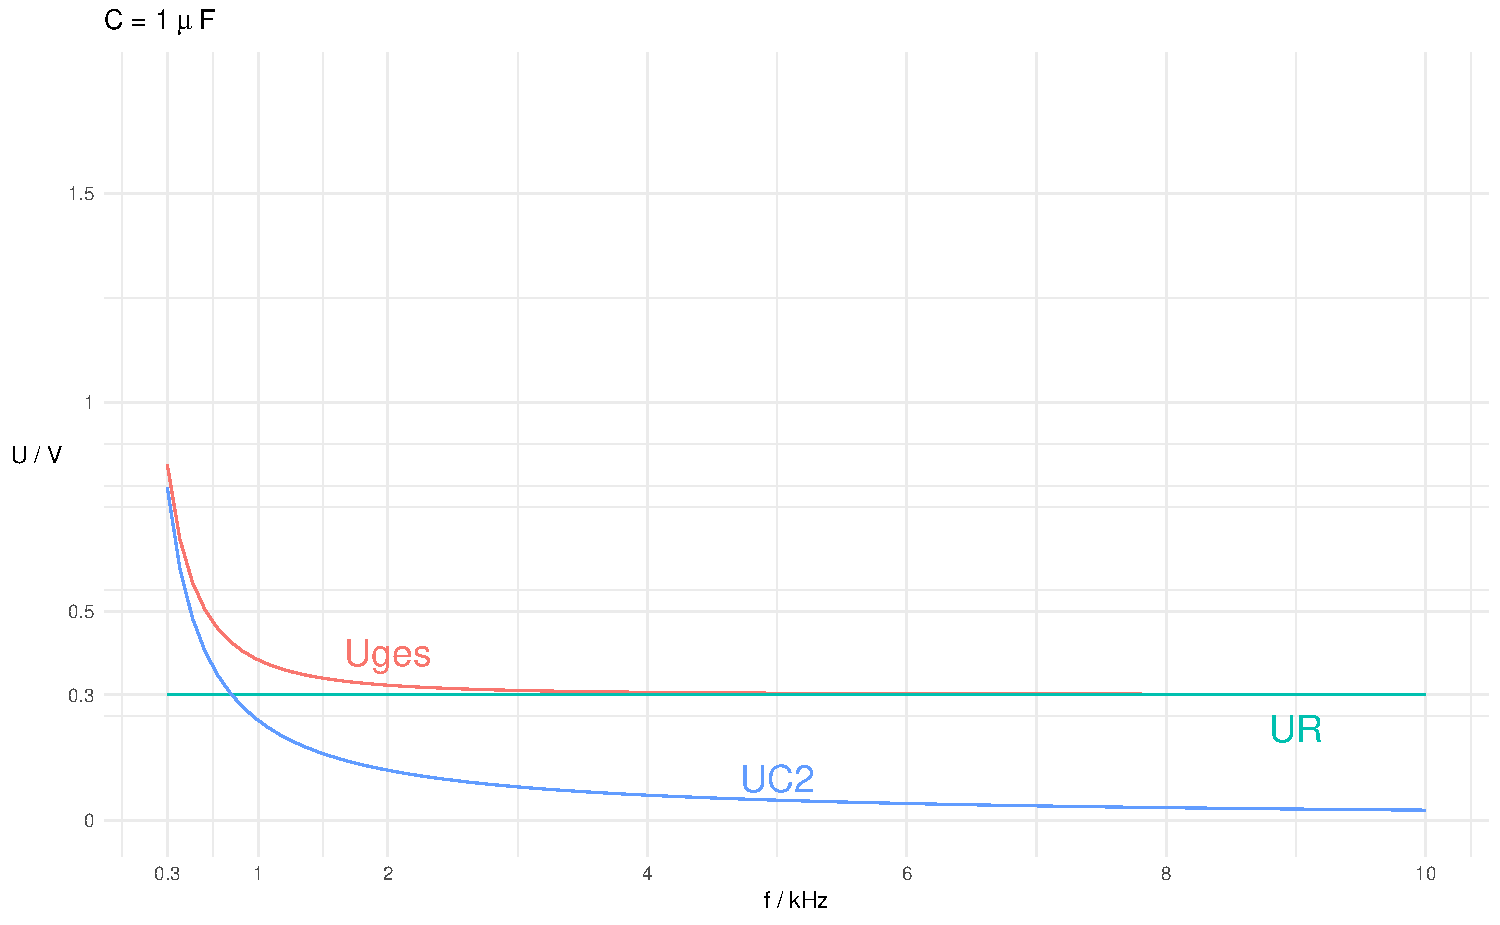
\includegraphics[scale=0.5]{./R/2_4/2_4_2.pdf}
    \end{center}

  %1.5
  \subsection{}
    \subsubsection*{a) Spule}

      %%%%%%%%%%%%%%%%%%%%%%%%%%%%%%%%%%%%%%%%%%%%%
        \begin{center}
          \begin{circuitikz}

            \draw (0,0) to[R, l=$R_{sL}$, o-] (2,0)
            to[L, l=$L_s$, -o] (4,0);

          \end{circuitikz}
        \end{center}
        \vspace{0.021276873\paperheight}

        \begin{center}
          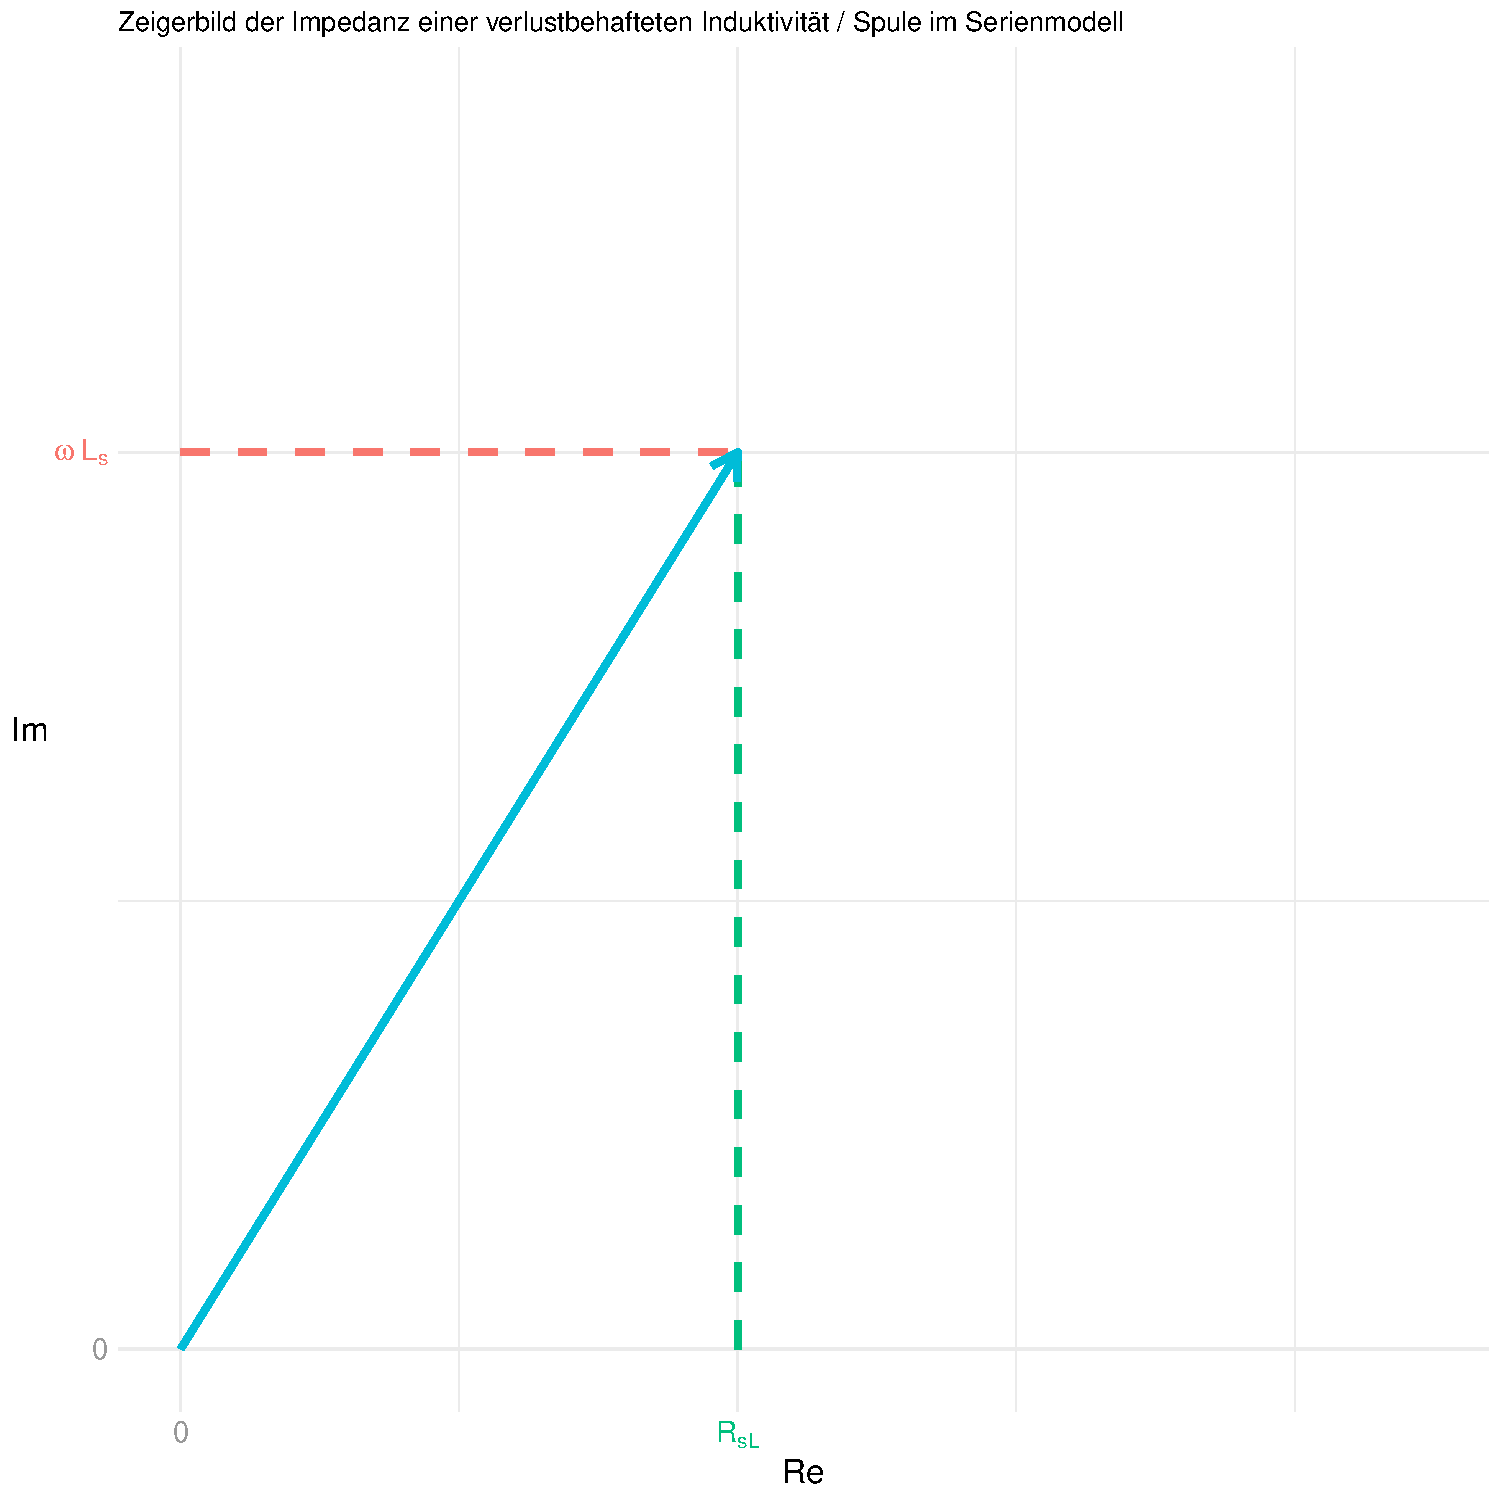
\includegraphics[scale=0.5]{./R/2_5/RL_Zeiger.pdf}
        \end{center}

        Der Winkel $\delta$, den die Impedanz $\underline{Z}$ mit der imaginären Achse bildet, wird Verlustwinkel genannt. Der Verlustfaktor $d$ ergibt sich dann aus:
        $$d = \tan{\delta} = \frac{R_{sL}}{L_s} $$

        \noindent Die Güte $Q$ ist definiert als der Kehrwert des Verlustfaktors, also:
        $$Q_{Ls} = \frac{1}{d} = \frac{\omega L_s}{R_{sL}} $$


      %%%%%%%%%%%%%%%%%%%%%%%%%%%%%%%%%%%%%%%%%%%%%
        \vspace{0.021276873\paperheight}
        \begin{center}
          \begin{circuitikz}

            \draw (0,0) -- (1,0);
            \draw (1,-1) -- (1,1);
            \draw (1,1) to[R, l=$R_{pL}$] (4,1);
            \draw (1,-1) to[L, l=$L_p$] (4,-1);
            \draw (4,-1) -- (4,1);
            \draw (4,0) -- (5,0);


          \end{circuitikz}
        \end{center}
        \vspace{0.021276873\paperheight}

        \begin{center}
          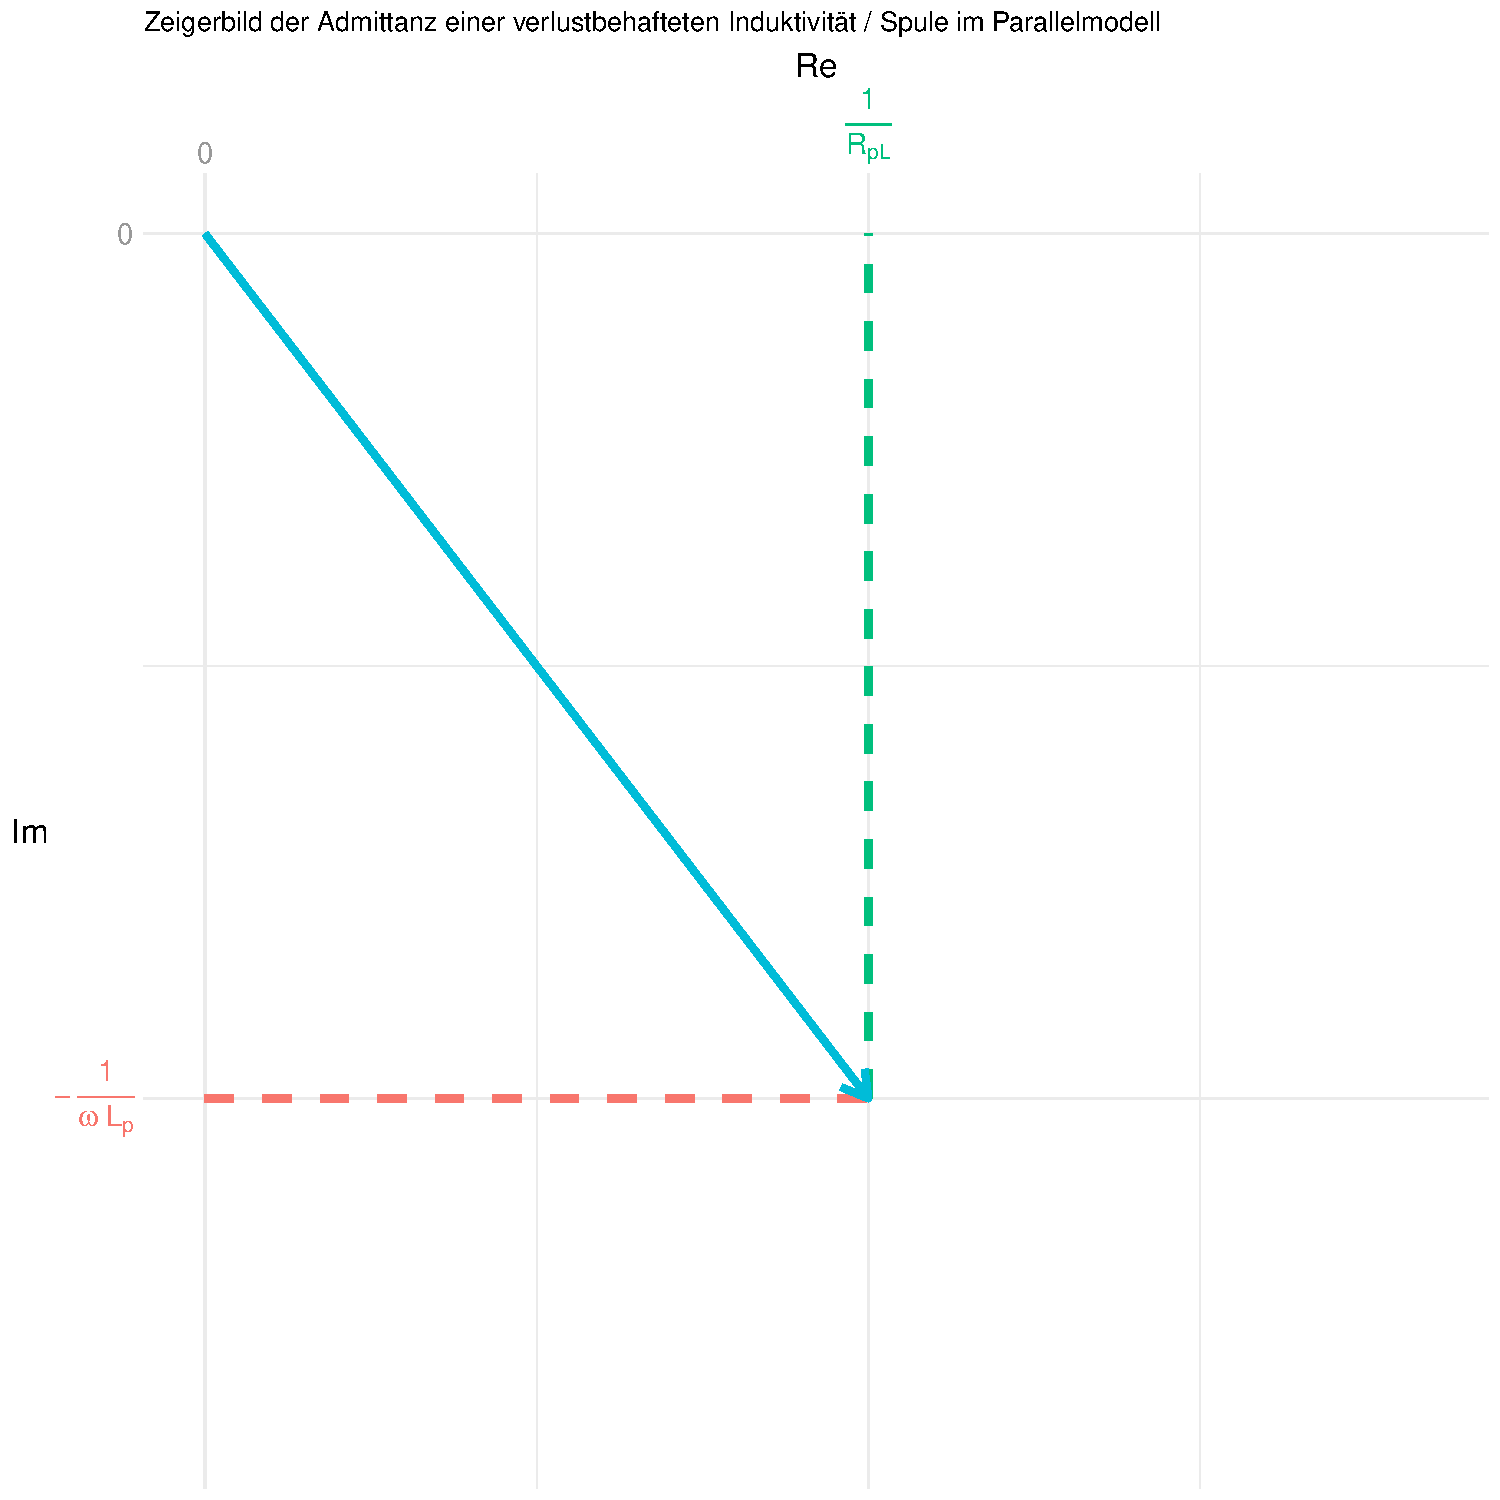
\includegraphics[scale=0.5]{./R/2_5/RL_Zeiger_parallel.pdf}
        \end{center}

        Analog ist der Verlustwinkel $\delta$ der Winkel der Admittanz mit der imaginären Achse:
        $$ d = \tan{\delta} = \frac{ \frac{1}{R_{pL}} }{ \mid - \frac{1}{\omega L_p} \mid} = \frac{\omega L_p}{R_{pL}} $$

        \noindent Demnach ist auch die Güte der Kehrwert des Verlustfaktors:
        $$Q_{Lp} = \frac{1}{d} = \frac{R_{pL}}{\omega L_p} $$

        \noindent Für die gleich Frequenz gilt damit:
        $$Q_{L_s} = Q_{L_p} = Q_L$$
      %%%%%%%%%%%%%%%%%%%%%%%%%%%%%%%%%%%%%%%%%%%%%

    \subsubsection*{b) Kondensator}

      \begin{center}
        \begin{circuitikz}

          \draw (0,0) to[R, l=$R_{sC}$, o-] (2,0)
          to[C, l=$C_s$, -o] (4,0);

        \end{circuitikz}
      \end{center}
      \vspace{0.021276873\paperheight}

      %%%%%%%%%%%%%%%%%%%%%%%%%%%%%%%%%%%%%%%%%%%%%
      \vspace{0.021276873\paperheight}
      \begin{center}
        \begin{circuitikz}

          \draw (0,0) -- (1,0);
          \draw (1,-1) -- (1,1);
          \draw (1,1) to[R, l=$R_{pC}$] (4,1);
          \draw (1,-1) to[C, l=$C_p$] (4,-1);
          \draw (4,-1) -- (4,1);
          \draw (4,0) -- (5,0);

        \end{circuitikz}
      \end{center}
      \vspace{0.021276873\paperheight}
      %%%%%%%%%%%%%%%%%%%%%%%%%%%%%%%%%%%%%%%%%%%%%

\section{Versuchsaufgaben}

\end{document}
